%\let\uppercase\relax

\vspace{24pt}

\chapter[\textbf{Constructing a Laser Profile}]{Constructing a Laser Profile}

Shock ignition involves aligning shockwaves so that they coalesce at the center of a target.  Because these shockwaves are the result of fluctuations in laser power, the laser profile containing these fluctuations must be constructed with a thorough and robust algorithm.  

As shown in Fig.\,\ref{fig:profConst}, there are six different laser pulses that constitute a shock ignition laser profile: a picket pulse, three pedestal pulses, a compression pulse, and an igniter pulse.  In terms of comparing shock ignition to other forms of ignition, the compression pulse and igniter pulse are the major differences, when it comes to power considerations.

\sidecaptionvpos{figure}{c}

\begin{SCfigure}[][h!]	
	\centering
	\caption[A Laser Power versus Time Profile]{ An Example Laser \\ Power versus Time Profile. \\ \captiontitlefinal{\textmd{A laser power versus time profile for shock ignition has six individual pulses.  It has: an initial picket pulse to develop a plasma envelope surrounding the target, three pedestal pulses to increase the target's density, a compression pulse, and a final igniter pulse \citep{terryThesis}. } } }
	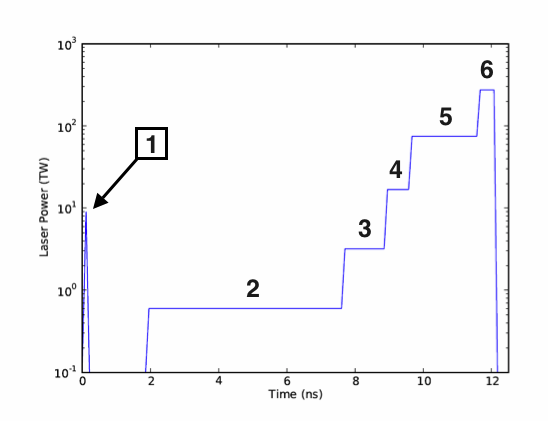
\includegraphics[scale=0.9]{graphics/profConst.png} 
	\label{fig:profConst}
\end{SCfigure}

\sidecaptionvpos{figure}{b}

  \section{Imposing a Picket Pulse}

The picket pulse`s main goal is to set the initial conditions of the simulation correctly.  Before the target is irradiated, it is a cryogenic piece of Hydrogen enclosed by a plastic shell.  The picket pulse is used to develop a plasma envelope surrounding the target.

This plasma envelope is useful for several reasons.  First, it increases the uniformity of laser absorption, which increases the spherical symmetry of the problem \citep{terryPaper}.  Second, it decreases the rate of instability growth on the shell`s surface, see Fig.\,\ref{fig:picketEffect}.  

\sidecaptionvpos{figure}{c}

\begin{SCfigure}[][h!]	
	\centering
	\caption[The Picket Pulse]{The Picket Pulse \\ \captiontitlefinal{\textmd{is designed to reduce the growth of Rayleigh-Taylor Instabilities (RTIs).  In this figure, the simulated RTI growth rate is taken as the linear growth rate in the 1.5 second window following the convergence of the three pedestal pulses at the ice-gas Hydrogen boundary for a wide range of mode numbers \citep{picketPaper}. } } }
	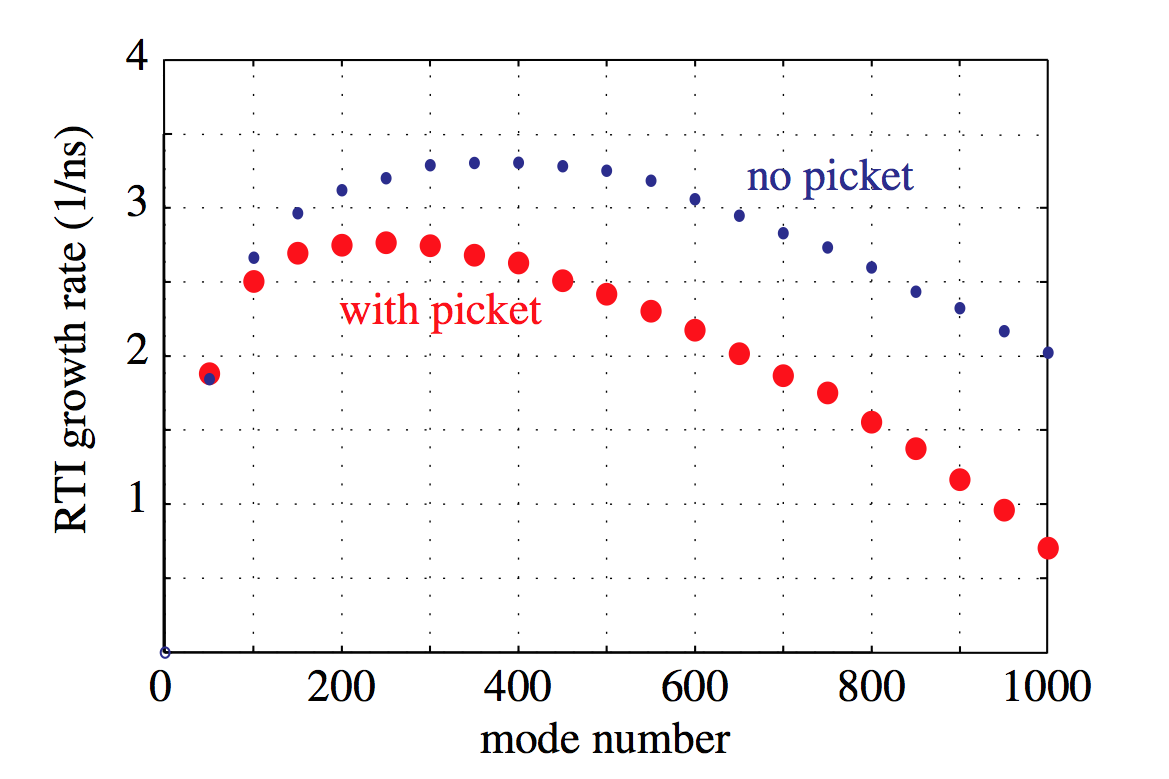
\includegraphics[width=0.55\textwidth]{graphics/picketEffect.png} 
	\label{fig:picketEffect}
\end{SCfigure}

\sidecaptionvpos{figure}{b}

  \section{Setting up Pedestal Pulses}
  \label{sec:pedestal}
The goal of the pedestal pulses is to increase the target`s fuel density by a factor of thirty, with a minimal amount of compression in the target. There are three pedestal pulses because each resulting shock is only theoretically capable of increasing the fuel density by a factor of four. Therefore, to achieve the sought after factor of thirty increase in fuel density, a minimum of three consecutive pulses are needed \citep{terryThesis}.  

To maximize the energy gain, the pedestal pulses need to be timed so that their resulting shockwaves arrive at the interface that exists between the outer Hydrogen ice shell and the inner Hydrogen gas region within fifty picoseconds of each other.  This interface is the optimum location for two reasons.  First, if the shockwaves were to pass each other within the Hydrogen ice region, they would cause unnecessary shock heating of the fuel.  Second, if the pulses were to meet inside the Hydrogen gas region, they would cause the fuel to decompress, which would be counter-productive to the process \citep{resultsVsSims}.

\section{Optimizing the Compression and Igniter Pulses}
\label{sec:mainPulses}
After the target`s density has increased by a factor of thirty, two more pulses are needed: the compression pulse and the igniter pulse.  Where constructing the picket pulse and the pedestal pulses required coalescing the resulting shockwaves at a single location, constructing the main pulses involves optimizing certain variables.  For the compression pulse, the maximized variable is the target`s density; for the igniter pulse, the maximized variable is the energy yield \citep{terryThesis}.
